
%% bare_jrnl_comsoc.tex
%% V1.4b
%% 2015/08/26
%% by Michael Shell
%% see http://www.michaelshell.org/
%% for current contact information.
%%
%% This is a skeleton file demonstrating the use of IEEEtran.cls
%% (requires IEEEtran.cls version 1.8b or later) with an IEEE
%% Communications Society journal paper.
%%
%% Support sites:
%% http://www.michaelshell.org/tex/ieeetran/
%% http://www.ctan.org/pkg/ieeetran
%% and
%% http://www.ieee.org/

%%*************************************************************************
%% Legal Notice:
%% This code is offered as-is without any warranty either expressed or
%% implied; without even the implied warranty of MERCHANTABILITY or
%% FITNESS FOR A PARTICULAR PURPOSE! 
%% User assumes all risk.
%% In no event shall the IEEE or any contributor to this code be liable for
%% any damages or losses, including, but not limited to, incidental,
%% consequential, or any other damages, resulting from the use or misuse
%% of any information contained here.
%%
%% All comments are the opinions of their respective authors and are not
%% necessarily endorsed by the IEEE.
%%
%% This work is distributed under the LaTeX Project Public License (LPPL)
%% ( http://www.latex-project.org/ ) version 1.3, and may be freely used,
%% distributed and modified. A copy of the LPPL, version 1.3, is included
%% in the base LaTeX documentation of all distributions of LaTeX released
%% 2003/12/01 or later.
%% Retain all contribution notices and credits.
%% ** Modified files should be clearly indicated as such, including  **
%% ** renaming them and changing author support contact information. **
%%*************************************************************************


% *** Authors should verify (and, if needed, correct) their LaTeX system  ***
% *** with the testflow diagnostic prior to trusting their LaTeX platform ***
% *** with production work. The IEEE's font choices and paper sizes can   ***
% *** trigger bugs that do not appear when using other class files.       ***                          ***
% The testflow support page is at:
% http://www.michaelshell.org/tex/testflow/



\documentclass[journal,comsoc]{IEEEtran}
%
% If IEEEtran.cls has not been installed into the LaTeX system files,
% manually specify the path to it like:
% \documentclass[journal,comsoc]{../sty/IEEEtran}


\usepackage[T1]{fontenc}% optional T1 font encoding


% Some very useful LaTeX packages include:
% (uncomment the ones you want to load)






\usepackage[pdftex]{graphicx}
\usepackage{pgfplots}
\usepackage{pgfplotstable}
\pgfplotsset{compat=1.9}




% *** MATH PACKAGES ***
%
\usepackage{amsmath}
% A popular package from the American Mathematical Society that provides
% many useful and powerful commands for dealing with mathematics.
% Do NOT use the amsbsy package under comsoc mode as that feature is
% already built into the Times Math font (newtxmath, mathtime, etc.).
% 
% Also, note that the amsmath package sets \interdisplaylinepenalty to 10000
% thus preventing page breaks from occurring within multiline equations. Use:
\interdisplaylinepenalty=2500
% after loading amsmath to restore such page breaks as IEEEtran.cls normally
% does. amsmath.sty is already installed on most LaTeX systems. The latest
% version and documentation can be obtained at:
% http://www.ctan.org/pkg/amsmath


% Select a Times math font under comsoc mode or else one will automatically
% be selected for you at the document start. This is required as Communications
% Society journals use a Times, not Computer Modern, math font.
\usepackage[cmintegrals]{newtxmath}
% The freely available newtxmath package was written by Michael Sharpe and
% provides a feature rich Times math font. The cmintegrals option, which is
% the default under IEEEtran, is needed to get the correct style integral
% symbols used in Communications Society journals. Version 1.451, July 28,
% 2015 or later is recommended. Also, do *not* load the newtxtext.sty package
% as doing so would alter the main text font.
% http://www.ctan.org/pkg/newtx
%
% Alternatively, you can use the MathTime commercial fonts if you have them
% installed on your system:
%\usepackage{mtpro2}
%\usepackage{mt11p}
%\usepackage{mathtime}


%\usepackage{bm}
% The bm.sty package was written by David Carlisle and Frank Mittelbach.
% This package provides a \bm{} to produce bold math symbols.
% http://www.ctan.org/pkg/bm





% *** SPECIALIZED LIST PACKAGES ***
%
\usepackage{algorithmic}
% algorithmic.sty was written by Peter Williams and Rogerio Brito.
% This package provides an algorithmic environment fo describing algorithms.
% You can use the algorithmic environment in-text or within a figure
% environment to provide for a floating algorithm. Do NOT use the algorithm
% floating environment provided by algorithm.sty (by the same authors) or
% algorithm2e.sty (by Christophe Fiorio) as the IEEE does not use dedicated
% algorithm float types and packages that provide these will not provide
% correct IEEE style captions. The latest version and documentation of
% algorithmic.sty can be obtained at:
% http://www.ctan.org/pkg/algorithms
% Also of interest may be the (relatively newer and more customizable)
% algorithmicx.sty package by Szasz Janos:
% http://www.ctan.org/pkg/algorithmicx




% *** ALIGNMENT PACKAGES ***
%
%\usepackage{array}
% Frank Mittelbach's and David Carlisle's array.sty patches and improves
% the standard LaTeX2e array and tabular environments to provide better
% appearance and additional user controls. As the default LaTeX2e table
% generation code is lacking to the point of almost being broken with
% respect to the quality of the end results, all users are strongly
% advised to use an enhanced (at the very least that provided by array.sty)
% set of table tools. array.sty is already installed on most systems. The
% latest version and documentation can be obtained at:
% http://www.ctan.org/pkg/array


% IEEEtran contains the IEEEeqnarray family of commands that can be used to
% generate multiline equations as well as matrices, tables, etc., of high
% quality.


\usepackage{listings}


% *** SUBFIGURE PACKAGES ***
%\ifCLASSOPTIONcompsoc
%  \usepackage[caption=false,font=normalsize,labelfont=sf,textfont=sf]{subfig}
%\else
%  \usepackage[caption=false,font=footnotesize]{subfig}
%\fi
% subfig.sty, written by Steven Douglas Cochran, is the modern replacement
% for subfigure.sty, the latter of which is no longer maintained and is
% incompatible with some LaTeX packages including fixltx2e. However,
% subfig.sty requires and automatically loads Axel Sommerfeldt's caption.sty
% which will override IEEEtran.cls' handling of captions and this will result
% in non-IEEE style figure/table captions. To prevent this problem, be sure
% and invoke subfig.sty's "caption=false" package option (available since
% subfig.sty version 1.3, 2005/06/28) as this is will preserve IEEEtran.cls
% handling of captions.
% Note that the Computer Society format requires a larger sans serif font
% than the serif footnote size font used in traditional IEEE formatting
% and thus the need to invoke different subfig.sty package options depending
% on whether compsoc mode has been enabled.
%
% The latest version and documentation of subfig.sty can be obtained at:
% http://www.ctan.org/pkg/subfig




% *** FLOAT PACKAGES ***
%
%\usepackage{fixltx2e}
% fixltx2e, the successor to the earlier fix2col.sty, was written by
% Frank Mittelbach and David Carlisle. This package corrects a few problems
% in the LaTeX2e kernel, the most notable of which is that in current
% LaTeX2e releases, the ordering of single and double column floats is not
% guaranteed to be preserved. Thus, an unpatched LaTeX2e can allow a
% single column figure to be placed prior to an earlier double column
% figure.
% Be aware that LaTeX2e kernels dated 2015 and later have fixltx2e.sty's
% corrections already built into the system in which case a warning will
% be issued if an attempt is made to load fixltx2e.sty as it is no longer
% needed.
% The latest version and documentation can be found at:
% http://www.ctan.org/pkg/fixltx2e


%\usepackage{stfloats}
% stfloats.sty was written by Sigitas Tolusis. This package gives LaTeX2e
% the ability to do double column floats at the bottom of the page as well
% as the top. (e.g., "\begin{figure*}[!b]" is not normally possible in
% LaTeX2e). It also provides a command:
%\fnbelowfloat
% to enable the placement of footnotes below bottom floats (the standard
% LaTeX2e kernel puts them above bottom floats). This is an invasive package
% which rewrites many portions of the LaTeX2e float routines. It may not work
% with other packages that modify the LaTeX2e float routines. The latest
% version and documentation can be obtained at:
% http://www.ctan.org/pkg/stfloats
% Do not use the stfloats baselinefloat ability as the IEEE does not allow
% \baselineskip to stretch. Authors submitting work to the IEEE should note
% that the IEEE rarely uses double column equations and that authors should try
% to avoid such use. Do not be tempted to use the cuted.sty or midfloat.sty
% packages (also by Sigitas Tolusis) as the IEEE does not format its papers in
% such ways.
% Do not attempt to use stfloats with fixltx2e as they are incompatible.
% Instead, use Morten Hogholm'a dblfloatfix which combines the features
% of both fixltx2e and stfloats:
%
% \usepackage{dblfloatfix}
% The latest version can be found at:
% http://www.ctan.org/pkg/dblfloatfix




%\ifCLASSOPTIONcaptionsoff
%  \usepackage[nomarkers]{endfloat}
% \let\MYoriglatexcaption\caption
% \renewcommand{\caption}[2][\relax]{\MYoriglatexcaption[#2]{#2}}
%\fi
% endfloat.sty was written by James Darrell McCauley, Jeff Goldberg and 
% Axel Sommerfeldt. This package may be useful when used in conjunction with 
% IEEEtran.cls'  captionsoff option. Some IEEE journals/societies require that
% submissions have lists of figures/tables at the end of the paper and that
% figures/tables without any captions are placed on a page by themselves at
% the end of the document. If needed, the draftcls IEEEtran class option or
% \CLASSINPUTbaselinestretch interface can be used to increase the line
% spacing as well. Be sure and use the nomarkers option of endfloat to
% prevent endfloat from "marking" where the figures would have been placed
% in the text. The two hack lines of code above are a slight modification of
% that suggested by in the endfloat docs (section 8.4.1) to ensure that
% the full captions always appear in the list of figures/tables - even if
% the user used the short optional argument of \caption[]{}.
% IEEE papers do not typically make use of \caption[]'s optional argument,
% so this should not be an issue. A similar trick can be used to disable
% captions of packages such as subfig.sty that lack options to turn off
% the subcaptions:
% For subfig.sty:
% \let\MYorigsubfloat\subfloat
% \renewcommand{\subfloat}[2][\relax]{\MYorigsubfloat[]{#2}}
% However, the above trick will not work if both optional arguments of
% the \subfloat command are used. Furthermore, there needs to be a
% description of each subfigure *somewhere* and endfloat does not add
% subfigure captions to its list of figures. Thus, the best approach is to
% avoid the use of subfigure captions (many IEEE journals avoid them anyway)
% and instead reference/explain all the subfigures within the main caption.
% The latest version of endfloat.sty and its documentation can obtained at:
% http://www.ctan.org/pkg/endfloat
%
% The IEEEtran \ifCLASSOPTIONcaptionsoff conditional can also be used
% later in the document, say, to conditionally put the References on a 
% page by themselves.




% *** PDF, URL AND HYPERLINK PACKAGES ***
%
%\usepackage{url}
% url.sty was written by Donald Arseneau. It provides better support for
% handling and breaking URLs. url.sty is already installed on most LaTeX
% systems. The latest version and documentation can be obtained at:
% http://www.ctan.org/pkg/url
% Basically, \url{my_url_here}.




% *** Do not adjust lengths that control margins, column widths, etc. ***
% *** Do not use packages that alter fonts (such as pslatex).         ***
% There should be no need to do such things with IEEEtran.cls V1.6 and later.
% (Unless specifically asked to do so by the journal or conference you plan
% to submit to, of course. )

\lstset{basicstyle=\ttfamily}


% correct bad hyphenation here
\hyphenation{op-tical net-works semi-conduc-tor}

\usepackage[backend=biber]{biblatex}
\addbibresource{refs.bib}


\begin{document}
%
% paper title
% Titles are generally capitalized except for words such as a, an, and, as,
% at, but, by, for, in, nor, of, on, or, the, to and up, which are usually
% not capitalized unless they are the first or last word of the title.
% Linebreaks \\ can be used within to get better formatting as desired.
% Do not put math or special symbols in the title.
\title{Deoptimisation support in MysoreScript}
%
%
% author names and IEEE memberships
% note positions of commas and nonbreaking spaces ( ~ ) LaTeX will not break
% a structure at a ~ so this keeps an author's name from being broken across
% two lines.
% use \thanks{} to gain access to the first footnote area
% a separate \thanks must be used for each paragraph as LaTeX2e's \thanks
% was not built to handle multiple paragraphs
%

\author{Joshua Send \\ Trinity Hall}% <-this % stops a space
\date{\today}

\maketitle

% As a general rule, do not put math, special symbols or citations
% in the abstract or keywords.
\begin{abstract}
Mysorescript is a simple scripting language which emulates basic Javascript. It is primarily interpreted, but has support for method-granularity just-in-time compilation using LLVM. While this offers large speed gains in many cases, code compiled at runtime is immutable. Addressing this fundamental point requires implementing deoptimisation, the process of modifying or replacing the compiled code to better utilize new runtime information. This report discusses deoptimisation for MysoreScript and evaluates it within the context of call-site inline caching.
\end{abstract}





% For peer review papers, you can put extra information on the cover
% page as needed:
% \ifCLASSOPTIONpeerreview
% \begin{center} \bfseries EDICS Category: 3-BBND \end{center}
% \fi
%
% For peerreview papers, this IEEEtran command inserts a page break and
% creates the second title. It will be ignored for other modes.
\IEEEpeerreviewmaketitle



\section{Introduction}

\IEEEPARstart{J}{ust} in time (JIT) compilation is an old technique which combines interpretation, and static ahead-of-time compilation. By initiating computation in the interpreter, the system can achieve fast startup times; selectively compiling oft-used code paths can then be used to improve execution speeds, thus combining some of the best parts of both approaches. The idea dates back to the 1960s, with LISP and later Smalltalk \cite{aycock2003brief} \cite{mccarthy1960recursive}.

One downside to running statically compiled software is that it cannot adapt and optimize in relation to the current system load, while a runtime which includes a JIT and a deoptimiser can dynamically recompile according to runtime information. Thus, JIT compilation may at some point be able to run more quickly than statically compiled code. The MysoreScript language includes only a JIT, so it is bound to provide bad compiled code in some situations. This report discusses the inclusion of deoptimisation in Mysorescript.


\subsection{MysoreScript Summary}
MysoreScript utilizes a parser which produces an actual abstract syntax tree (AST), with nodes in the tree represented by classes. The runtime initiates interpretation starting at the root block of statements, recursively evaluating each child of the root. In effect, the interpreter is performing a depth-first execution. The use of classes to define AST nodes, each with their own \lstinline|interpret| method induces a call stack, which will have to be rebuilt when resuming execution in the interpreter (Section \ref{sec:deoptimisation:jitandback}).

Another relevant feature of the language is that all closures, methods and functions are represented as the same object but with different calls for interpretation and compilation. This type of object is the unit of AST compilation, since the language only supports method-granularity compilation. Bound variables for closures are handled by copy, rather than reference: on creation of a closure the value of outer bound variables are copied into inner symbol tables.

Compilation is always initiated from the interpreter, which calls either a \lstinline|compileMethod| or \lstinline|compiledClosure| and saves the resulting compiled function. Because sub-calls within a function are not necessarily also compiled, a series of trampolines provide support for calling into the interpreter from the compiled functions.

\subsection{Report Outline}

This report discusses the inclusion of deoptimisation to Mysorescript. The new functionality is evaluated with an implementation of inline caching, which includes type assumptions and method locations hardcoded into the fast path. The following sections discuss deoptimisation, inline caching, and an evaluation in turn.


\section{Deoptimisation}
\subsection{Overview} 

The key step to implementing deoptimization is the being able to exit a compiled function and resume execution in the interpreter, if a slow path is hit (that is, some kind of compile time assumption is invalidated). To be achieve this, stackmaps~\footnote{\url{https://llvm.org/docs/StackMaps.html}} can be used, which use a special data section of the compiled executable to record the value of variables. This section can be used to re-assemble an interpreter context with local, bound, and argument variables. 

Once the interpreter context has been reconstructed, an interpreter evaluation stack has to be re-created to perform the correct tree execution of the AST nodes starting from the node that execution was suspended at. A simplifying assumption, that execution only stops on statement boundaries, was made here. In practical terms, this requires that MysoreScript code be written in SSA-like forms.

Once the execution has been resumed and completed in the interpreter, the result of the function is passed back to the compiled code to return immediately.
	
\subsection{Resuming execution in the Interpreter}
	\subsubsection{Stackmaps and Patchpoints}
		Stackmaps are a program section emitted by the compiler which can be used to record a set of values or locations given at compile time. There are two LLVM intrinsics which initiate the creation of a Stackmap entry: \lstinline|llvm.experimental.stackmap| and \lstinline|llvm.experimental.patchpoint|, with the latter coming in \lstinline|void| and \lstinline|i64| (64 bit integer) return type variations.
		
\begin{lstlisting}[caption={Stackmap Section Layout}, label={lst:stackmap}, basicstyle=\footnotesize]
Header {
  uint8  : Stack Map Version (current is 3)
  uint8  : Reserved (expected to be 0)
  uint16 : Reserved (expected to be 0)
}
uint32 : NumFunctions
uint32 : NumConstants
uint32 : NumRecords
StkSizeRecord[NumFunctions] {
  uint64 : Function Address
  uint64 : Stack Size
  uint64 : Record Count
}
Constants[NumConstants] {
  uint64 : LargeConstant
}
StkMapRecord[NumRecords] {
  uint64 : PatchPoint ID
  uint32 : Instruction Offset
  uint16 : Reserved (record flags)
  uint16 : NumLocations
  Location[NumLocations] {
    uint8  : Register | Direct | ...
    uint8  : Reserved (expected to be 0)
    uint16 : Location Size
    uint16 : Dwarf RegNum
    uint16 : Reserved (expected to be 0)
    int32  : Offset or SmallConstant
  }
  uint32 : Padding (only if not 8byte aligned)
  uint16 : Padding
  uint16 : NumLiveOuts
  LiveOuts[NumLiveOuts]
    uint16 : Dwarf RegNum
    uint8  : Reserved
    uint8  : Size in Bytes
  }
  uint32 : Padding (only if not 8byte aligned)
}
		\end{lstlisting}
		
		The \lstinline|stackmap| intrinsic only requires an ID and a list of values to record, which are saved into a stackmap section. The \lstinline|patchpoint| intrinsics take an ID, bytes to reserve for code patching (not used), a function to call, arguments to the function, and any values to save to the stackmap.
		
		In order to call back into the interpreter without causing disruption to the register allocation for the fast path in the compiled code, the \lstinline|AnyReg| calling convention (Section \ref{sec:deoptimisation:jitandback}) should be used -- this is only available with the \lstinline|patchpoint| intrinsic. Its return value will additionally be used to get the result of the function from the interpreter.
		
		Listing \ref{lst:stackmap} shows the memory layout of the stackmap section. Each function has an associated number of records, one per \lstinline|patchpoint| or \lstinline|stackmap| intrinsic. Due to the method-granularity compilation, a separate Stackmap section is emitted per method, and number of functions is always one.
		
		While it should be possible to have more than one \lstinline|StkMapRecord| per function, I failed to implement this as the value of the \lstinline|Function Address| was always 0. Normally, the way to find an the desired stackmap record is to calculate the $Function Address + Instruction Offset$ which should be equal to the return address of the intrinsic function call. Thus for evaluation I was forced to restrict myself to examples with a single call site per function.
		
		The \lstinline|patchpoint.i64| intrinsic stores arguments in a set of \lstinline|Location|'s, the first of which indicates the return register when using the AnyReg calling convention.
		
		To interface with a stackmap section easily, a \lstinline|StackMapParser| was created, which takes the address of the stackmap and returns saved values, transparently handling the raw memory addressing. 
		
		It is recommendable to save only live variables to the stack map. However, I ran out of time to implement this. Stackmap records already contain a set of live registers at the call site, but this would be difficult to match back to variable names. A live variable analysis could be written over the abstract syntax tree instead.
	 
	\subsubsection{Intercepting JIT Program Sections}
		To be able to initialize a \lstinline|StackMapParser| the address of the stackmap section is required. This was obtained by registering an event listener with the JIT execution engine. The callback receives a notification on each section created, but only the one named \lstinline|.llvm_stackmaps| is saved.
		
		Since multiple functions my be compiled and produce independent stackmap sections, the runtime maintains a mapping from compiled functions to the correct stackmap sections -- a side exit from a compiled method is not able to convey any immediate information to the callee when using the AnyReg calling convention.
		
		The first solution to this involved extending the built in, simple JIT memory manager to record section addresses, but this would not consistently operate correctly. A second, fully functional solution was built along the lines of Pyston's program section interceptor \footnote{Thanks to the now defunct Pyston! \url{https://github.com/dropbox/pyston}}.
	
	\subsubsection{JIT to Interpreter and Back} 
	\label{sec:deoptimisation:jitandback}
		
		The AnyReg calling convention was used to make the compiled fast path even more efficient. However, in contrast to the C System V x86\_64 calling convention, which assigns certain registers to be used as arguments, some as return holders, and some registers as caller- and callee-preserved, AnyReg preserves registers from before the call and places the burden of finding arguments to the function on the callee via the stackmap, which stores records in order of arguments.
		
		To deal with this, an x86-64 assembly trampoline was written, which pushes all registers onto the stack, and does a C style call into the interpreter function \lstinline|reconstructInterpreterContext|, passing the location of the registers pushed onto the stack. The interpreter then retrieves the current stackmap from the runtime, which keeps track of the running JIT'ed function via a simple pointer, and uses the stackmap record locations and the stack of register values to retrieve variables saved at the patchpoint location. These values are used to reconstruct a valid interpreter context. The \lstinline|resumeInInterpreter| function is then called.
		
	
		\begin{figure}[htb]
			\centering
			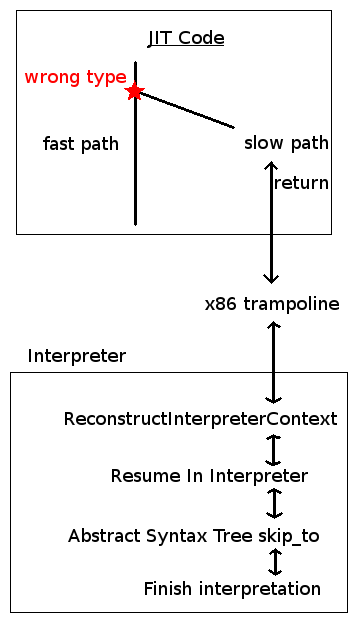
\includegraphics[width=6cm]{./Architecture.png}
			\caption{Program control flow when resuming in interpreter.}
			\label{fig:abc}
		\end{figure}
		
		Because the JIT'ed function is called with standard C calling conventions, it may have preserved caller registers that need to be recovered from the stack, while also retuning a value. To achieve this, the x86 trampoline places the return value from the interpreter resumption, into the register indicated by the first stackmap location. The JIT slow path then immediately returns this value.
		
		If there were no spilled variables, a faster method would be to have the x86 trampoline pop off the JIT stack frame, except the return address and jump or call into the \lstinline|resumeInInterpreter| function, which would return straight to the caller of the JIT function. This would provide speedups by not requiring passing return values back through various stack frames.
	
	\subsubsection{Skipping to correct AST Node}
		\lstinline|resumeInInterpreter| utilizes the pointer to the currently executing JIT'ed function, an AST node, as the root of a DFS tree search searching for the AST node execution was paused at. This was implemented by mirroring the \lstinline|interpret| methods on AST nodes, with some significant modifications. 
		
		The main task is retrieving the function value computed by the time a return statement is encountered. This may mean switching from skipping, and not executing commands while locating the desired AST node, to full interpretation. This is well exemplified in Listing \ref{lst:skipto}.
		
\begin{lstlisting}[caption={The skip\_to method on a block of Statements}, label={lst:skipto},basicstyle=\footnotesize]
void Statements::skip_to(Interpreter::Context &c, 
	Statement* ast_node) {                                          
  for (auto &s : statements) {                                                                                  
    if (c.isReturning) {                                                                                      
      return;  
    }            
    if (c.astNodeFound) {                                                                                     
      s->interpret(c);  
    } else{
      s->skip_to(c,ast_node);    
    } 
  }     
}    
\end{lstlisting}
	
	Return values and the flag for when to switch from skipping nodes to full interpretation are both attached to the interpreter context.
	
\subsection{Recompilation}
	\label{sec:recompilation}
	\subsubsection{Profiling}
		Another key element of the deoptimization process is the actual replacement of compiled functions. This requires some kind of profiling of the data. In this case, the focus is on inline caching.
		
		A simple replacement strategy was implemented using a \lstinline|current_type_assumption| pointer to a class attached to every call site (actually, every AST node inherits the same ability to set assumptions, and usable at compile time to optimize the fast path), a pointer to an alternative type, \lstinline|alternative_type|, and a counter \lstinline|alternative_type_count|.
		
		The simple algorithm used here is outlined in Listing \ref{lst:replacement}. This strategy requires at least $threshold$ contiguous alternative types to initiate a recompile. The effect of this value is explored in Section \ref{sec:threshold}
\begin{lstlisting}[caption={Recompilation Strategy Pseudocode}, label={lst:replacement},basicstyle=\footnotesize]
...
type = object->isa; // get the type
if type == current_type_assumption:
  alternative_type_count = 0
  ...execute fast path...
else:
  if type == alternative_type:
  	alternative_type_count++;
  	if alternative_type_count > threshold:
  	  set recompile flag on the current closure
  	  current_type_assumption = type
  	  alternative_type = nullptr
  	  alternative_type_count = 0
  else:
  	alternative_type = type
  	alternative_type_count = 0
  ... execute slow path...
\end{lstlisting}		

	More sophisticated schemes are possible that require more data to be collected lend themselves to heterogeneous, randomized mixtures of data types rather than the sequences of identical types optimized for here.
	
	\subsubsection{Recompilation and Replacement}
	Once the slow path has been taken often enough, on exit from the interpreter resumption back into the x86 trampoline, the \lstinline|recompile| flag is checked. If it is set, the current function being executed is checked for the presence of a selector to determine if needs to be compiled as a method, or as a closure, and the corresponding methods are called on the root AST node.
	
	The useful thing about embedding type assumptions in individual AST nodes mean that during their compilation, they can specialize their code based on those assumption, and by changing the assumptions in the interpreter and inducing recompilation, the changes are automatically incorporated. This in conjunction with callsite caching is explored in Section \ref{sec:inlcache}.
	
	I note here that the replacement may be causing memory leaks, as I do not free the memory used by previous recompilations. This would requires some effort, since the JIT function cannot be fully deleted until the x86 trampoline has returned to it, and it has returned again. However, with small functions such as the ones tested here, the memory leak is not an issue.


\section{Inline Callsite Caching}
\label{sec:inlcache}
	\subsection{Concept}
		Callsite inline caching saves a function pointer at each call site, which may be used if the desired method matches the type saved with the pointer. The policy for replacement of the pointer is also flexible. I use immediate replacement for testing.
		
		A simple, and effective implementation is to store a pointer to a type, and a pointer to a method at each call site in the AST. The interpreter can then use these to do caching, providing modest speedups if there are multiple methods attached to the target class (compare Figure \ref{fig:100kbase} to Figure \ref{fig:200methods}).
		
		The interpreter code can be directly translated into machine code during the compilation process, using pointers to the cached type and method pointers. The compiled method must check for null and special integer object types, but the slow path only does one method lookup and a store operation during a cache miss -- since the cache is updated immediately, this leads to a fast compiled code execution over relatively homogeneous data streams. The experiments carried out in the Evaluation section show this as well.
		
	\subsection{Using Deoptimisation}
	
		The callsite inline caching implementation is somewhat different with deoptimization, in that the fast path can be very short and hard code the expected type and location of the cached method, based on the \lstinline|current_type_assumption| value and the method looked up previously in the slow path.
		
		The compiler can even use the type information to generate specialized code based -- for instance, the \lstinline|SmallInteger| class would normally need to checked for by examining the lower 3 bits of a pointer. However, assuming it is an integer means this check can be avoided in the compiled code.

	
\section{Evaluation}
	
	This section will analyze the caching optimization implemented using various sample programs. Configurations explored are: adjusting the number of times a (potentially compiled) closure is called, the number of class methods present, and the number of different types a function is applied to, which in turn induces re-compilations if deoptimization is available. The programs using a mixture of types are implemented with long sequences of each type rather than a random stream to make better use of the recompilation strategy outlined in Section \ref{sec:recompilation}. 
	
	Comparisons to the original, unmodified MysoreScript code base, and to a inline callsite caching implementation following Section \ref{sec:inlcache} without deoptimization are provided. The focus is on execution time. Memory usage is extremely stable and sits around 108KB for non-JIT'ing configurations, and 126KB to 135KB for 1-5 JIT'ed functions.

	\subsection{Baseline}
	The first configuration tested is a program with a simple two-class hierarchy, with one function and one instance integer-value variable. The subclass overrides the parent's implementation of the function. An external $getter$ takes one of these two objects and calls the function, which simply returns the instance variable.
	
	Figure \ref{fig:100kbase} presents the result of evaluating the $getter$ 50,000 times with an instance of the parent, and 50,000 times with the sub-class. This induces a recompilation after a the side exit is taken too many times.
	
	\begin{figure}[htb]

	\caption{Running time for different MysoreScript configurations. The non-JIT'ing versions are in red and blue.}
	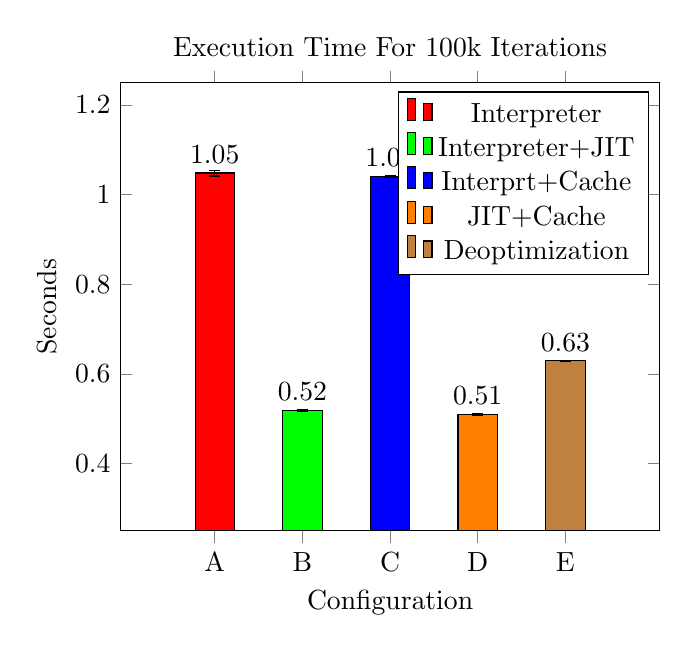
\begin{tikzpicture}
	\begin{axis}[
		ybar,
		title=Execution Time For 100k Iterations,
		xlabel={Configuration},
		ylabel={Seconds},
		ymin=0.25,
		ymax=1.25,
		symbolic x coords={A, B, C, D, E},
		xtick={A, B, C, D, E},
		bar width=0.5cm,                       %% changed
    	ybar=-0.5cm,                           %% new
    	enlarge x limits={abs=1.2cm},
    	nodes near coords, nodes near coords align={vertical},
	]
	\addplot[black, fill=red, error bars/.cd, y dir=both, y explicit] 
		coordinates {
		(A,1.048) += (0,0.0065) -= (0,0.0065)
		}; 
	\addplot[black, fill=green, error bars/.cd, y dir=both, y explicit] 
		coordinates {(B,0.5178) += (0,0.0022) -= (0,0.0022)}; 		
	\addplot[black, fill=blue, error bars/.cd, y dir=both, y explicit] 
		coordinates {(C,1.041) += (0,0.0017) -= (0,0.0017)}; 
	\addplot[black, fill=orange, error bars/.cd, y dir=both, y explicit] 
		coordinates {(D,0.509) += (0,0.0025) -= (0,0.0025)}; 
	\addplot[black, fill=brown, error bars/.cd, y dir=both, y explicit] 
		coordinates {(E,0.629) += (0,0.0016) -= (0,0.0016)}; 	
	\legend{Interpreter, Interpreter+JIT,Interprt+Cache, JIT+Cache, Deoptimization}
	\end{axis}
	\end{tikzpicture}
		\label{fig:100kbase}
	\end{figure}
	
	Things first thing to note here is that preventing MysoreScript from activating the JIT has severe performance penalty, of around 50-100\%. Further, caching has very little impact over simple compilation without it -- likely because only 1 function needs to be looked up using the $O(n)$ search strategy without it.
	
	Lastly, note that deoptimization decreases performance, by around 25\%. The difference in means between using the JIT+caching configuration and the deoptimizing configuration is $0.629216 - 0.5094416 = 0.1197744$ seconds. A measure of the time taken to execute a compilation of a simple function like the ones used here gives approximately $0.1486
	\pm0.005$ seconds. Thus the gap is attributed to the extra recompilation that needs to be done halfway through execution. We expect this gap to shrink as the iterations increase.

	
	\subsection{Increasing Number of Iterations}
	Increasing the number of iterations in the same program from 100,000 to 1 million illustrates the decreasing gap well. Non-JIT'ing configurations are left out here.
	
	\begin{figure}[htb]

	\caption{Running time for different JIT'ing configurations -- non compiling versions are left out here. 1 million iterations.}
	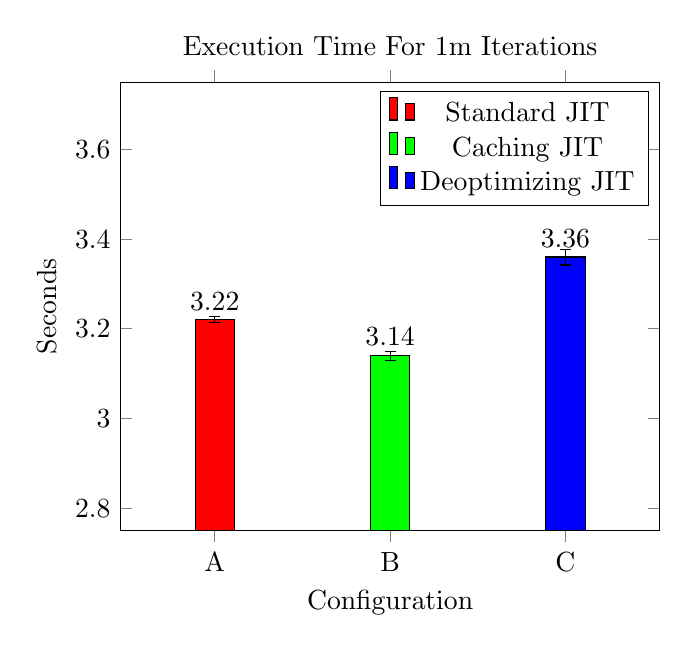
\begin{tikzpicture}
	\begin{axis}[
		ybar,
		title=Execution Time For 1m Iterations,
		xlabel={Configuration},
		ylabel={Seconds},
		ymin=2.75,
		ymax=3.75,
		symbolic x coords={A, B, C},
		xtick={A, B, C},
		bar width=0.5cm,                       %% changed
    	ybar=-0.5cm,                           %% new
    	enlarge x limits={abs=1.2cm},
    	nodes near coords, nodes near coords align={vertical},
	]
	\addplot[black, fill=red, error bars/.cd, y dir=both, y explicit] 
		coordinates {
		(A,3.22) += (0,	0.0064) -= (0,	0.0064)
		}; 
	\addplot[black, fill=green, error bars/.cd, y dir=both, y explicit] 
		coordinates {(B,3.14) += (0,0.0100) -= (0,0.0100)}; 		
	\addplot[black, fill=blue, error bars/.cd, y dir=both, y explicit] 
		coordinates {(C,3.36) += (0,0.0177) -= (0,0.0177)}; 
	
	\legend{Standard JIT, Caching JIT, Deoptimizing JIT}
	\end{axis}
	\end{tikzpicture}
		\label{fig:1m}
	\end{figure}
	
		Figure \ref{fig:1m} shows that all three of basic JIT, inline-caching JIT, and deoptimizing inline-caching are competitive with each other. The inline-caching JIT is slightly ahead of the others.

		
		\begin{figure}[htb]

		\caption{Running time for different JIT'ing configurations -- non compiling versions are left out here. 10 million iterations. Note the graph is plotting very similar values quite differently.}
		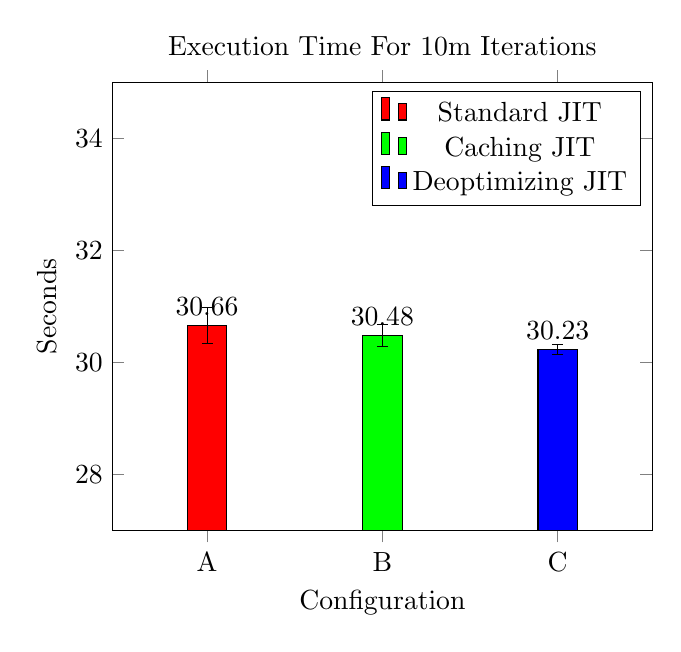
\begin{tikzpicture}
		\begin{axis}[
			ybar,
			title=Execution Time For 10m Iterations,
			xlabel={Configuration},
			ylabel={Seconds},
			ymin=27,
			ymax=35,
			symbolic x coords={A, B, C},
			xtick={A, B, C},
			bar width=0.5cm,                       %% changed
	    	ybar=-0.5cm,                           %% new
	    	enlarge x limits={abs=1.2cm},
	    	nodes near coords, nodes near coords align={vertical},
		]
		
		\addplot[black, fill=red, error bars/.cd, y dir=both, y explicit] 
			coordinates {
			(A, 30.66) += (0, 0.32) -= (0,0.32)
			}; 
		\addplot[black, fill=green, error bars/.cd, y dir=both, y explicit] 
			coordinates {(B,30.48) += (0,0.19) -= (0,0.19)}; 		
		\addplot[black, fill=blue, error bars/.cd, y dir=both, y explicit] 
			coordinates {(C, 30.23) += (0,0.085) -= (0,0.085)}; 
		
		\legend{Standard JIT, Caching JIT, Deoptimizing JIT}
		\end{axis}
		\end{tikzpicture}
				\label{fig:10m}
		\end{figure}
	

	Increasing the number of iterations (Figure \ref{fig:10m}) by another factor of 10 to 10 million leads to inconclusive results: all three configurations are within one standard deviation of each other. However, it is reassuring that the deoptimizing JIT is no slower than the others, and perhaps a more complete implementation would lead to statistically significant speed gains.
	
	\subsection{Increasing Number of Class Methods}
	The previous experiments were all done with a class hierarchy in which members had a single method. This is not only unrealistic, but favors the non-caching, standard language implementation without any profiling or instrumentation, as seen above.
	
	To look at an extreme first, the program is modified to include an extra 200 member functions in the parent class. Figure \ref{fig:200methods} shows the 100k iterations scenario again. The non-caching configurations are now noticably slower than the cahing ones, which have almost no performance penalty.
	
	\begin{figure}[htb]

	\caption{Running time for different JIT'ing configurations.}
	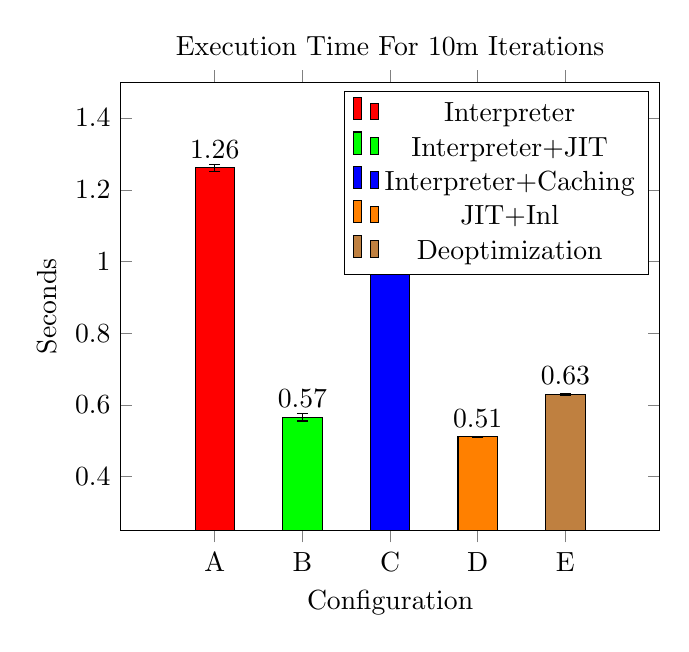
\begin{tikzpicture}
	\begin{axis}[
		ybar,
		title=Execution Time For 10m Iterations,
		xlabel={Configuration},
		ylabel={Seconds},
		ymin=0.25,
		ymax=1.5,
		symbolic x coords={A, B, C, D, E},
		xtick={A, B, C, D, E},
		bar width=0.5cm,                       %% changed
		ybar=-0.5cm,                           %% new
		enlarge x limits={abs=1.2cm},
		nodes near coords, nodes near coords align={vertical},
	]

	\addplot[black, fill=red, error bars/.cd, y dir=both, y explicit] 
		coordinates {
		(A, 1.260904) += (0, 0.01) -= (0,0.01)
		}; 
	\addplot[black, fill=green, error bars/.cd, y dir=both, y explicit] 
		coordinates {(B,0.565237) += (0,0.01) -= (0,0.01)}; 		
	\addplot[black, fill=blue, error bars/.cd, y dir=both, y explicit] 
		coordinates {(C, 1.093) += (0,0.01) -= (0,0.01)}; 
	\addplot[black, fill=orange, error bars/.cd, y dir=both, y explicit] 
		coordinates {(D,0.511) += (0,0.0015) -= (0,0.0015)}; 		
	\addplot[black, fill=brown, error bars/.cd, y dir=both, y explicit] 
		coordinates {(E, 0.63) += (0,0.0025) -= (0,0.0025)}; 
	\legend{Interpreter, Interpreter+JIT,Interpreter+Caching, JIT+Inl, Deoptimization}
	\end{axis}
	\end{tikzpicture}\\
		\label{fig:200methods}
	\end{figure}
			
	Here too one can watch the performance gap between caching JIT and deoptimizing+caching JIT shrink as the number of iterations is increased. Unfortunately the results between cachingng JIT and deoptimizing JIT (Figure \ref{fig:200methods_10miterations}, for 10 million iterations) are not statistically significant.
	
	\begin{figure}[htb]
	\caption{Running time for different JIT'ing configurations with 200 class methods and 1m iterations. Non-compiling configurations have been left out.}
	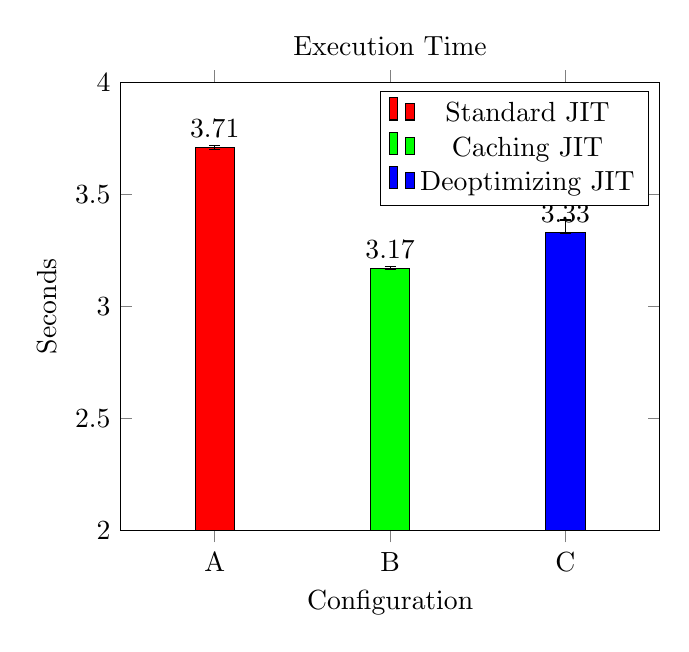
\begin{tikzpicture}
		\begin{axis}[
			ybar,
			title=Execution Time,
			xlabel={Configuration},
			ylabel={Seconds},
			ymin=2,
			ymax=4,
			symbolic x coords={A, B, C},
			xtick={A, B, C},
			bar width=0.5cm,                       %% changed
		   	ybar=-0.5cm,                           %% new
		   	enlarge x limits={abs=1.2cm},
		   	nodes near coords, nodes near coords align={vertical},
		]
	\addplot[black, fill=red, error bars/.cd, y dir=both, y explicit] 
		coordinates {
			(A, 3.71) += (0, 0.009) -= (0,0.009)
		}; 
	\addplot[black, fill=green, error bars/.cd, y dir=both, y explicit] 
		coordinates {(B,3.17) += (0,0.006) -= (0,0.006)}; 		
	\addplot[black, fill=blue, error bars/.cd, y dir=both, y explicit] 
		coordinates {(C, 3.33) += (0,0.055) -= (0,0.0055)}; 
		
	\legend{Standard JIT, Caching JIT, Deoptimizing JIT}
	\end{axis}
	\end{tikzpicture}
	
		\label{fig:200methods_1miterations}
	\end{figure}
	
	\begin{figure}[htb]

	\caption{Running time for different JIT'ing configurations with 200 class methods and 10m iterations. Non-compiling configurations have been left out.}
	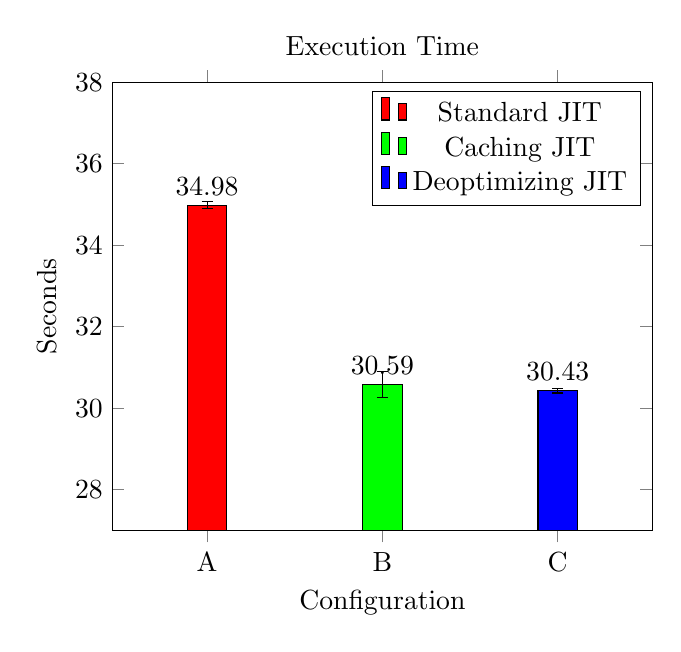
\begin{tikzpicture}
		\begin{axis}[
			ybar,
			title=Execution Time,
			xlabel={Configuration},
			ylabel={Seconds},
			ymin=27,
			ymax=38,
			symbolic x coords={A, B, C},
			xtick={A, B, C},
			bar width=0.5cm,                       %% changed
		   	ybar=-0.5cm,                           %% new
		   	enlarge x limits={abs=1.2cm},
		   	nodes near coords, nodes near coords align={vertical},
		]
	\addplot[black, fill=red, error bars/.cd, y dir=both, y explicit] 
		coordinates {
			(A, 34.98) += (0, 0.09) -= (0,0.09)
		}; 
	\addplot[black, fill=green, error bars/.cd, y dir=both, y explicit] 
		coordinates {(B,30.59) += (0,0.32) -= (0,0.32)}; 		
	\addplot[black, fill=blue, error bars/.cd, y dir=both, y explicit] 
		coordinates {(C,30.43) += (0,0.055) -= (0,0.055)}; 
		
	\legend{Standard JIT, Caching JIT, Deoptimizing JIT}
	\end{axis}
	\end{tikzpicture}
		\label{fig:200methods_10miterations}
	\end{figure}	
		
	The same game can be played with 20, rather than 200 class methods: this is a much more realistic scenario, though languages like Java with large class hierarchies may exceed that number easily. Only the 10 million iteration data is plotted here to reduce clutter. See Figure \ref{fig:20methods_10miterations}.
		\begin{figure}[htb]

		\caption{Running time for different JIT'ing configurations with 20 class methods and 10m iterations. Non-compiling configurations have been left out.}
		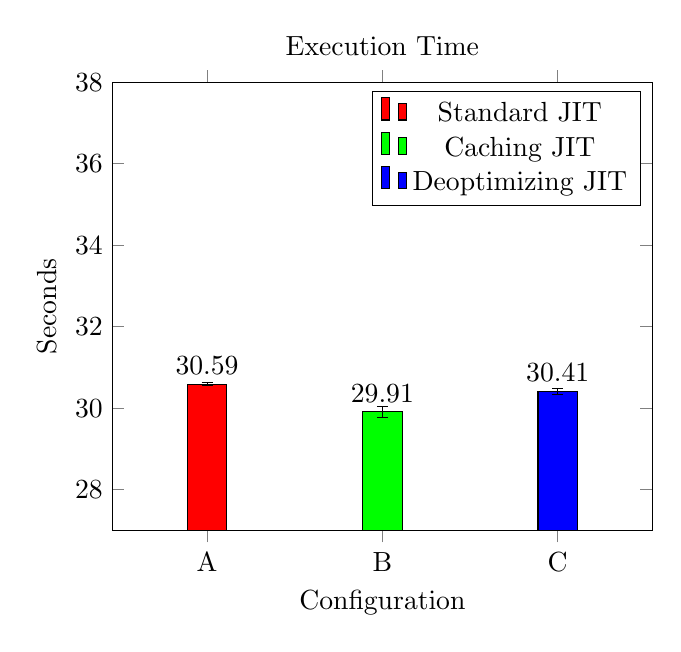
\begin{tikzpicture}
			\begin{axis}[
				ybar,
				title=Execution Time,
				xlabel={Configuration},
				ylabel={Seconds},
				ymin=27,
				ymax=38,
				symbolic x coords={A, B, C},
				xtick={A, B, C},
				bar width=0.5cm,                       %% changed
			   	ybar=-0.5cm,                           %% new
			   	enlarge x limits={abs=1.2cm},
			   	nodes near coords, nodes near coords align={vertical},
			]
		\addplot[black, fill=red, error bars/.cd, y dir=both, y explicit] 
			coordinates {
				(A, 30.59) += (0, 0.04) -= (0,0.04)
			}; 
		\addplot[black, fill=green, error bars/.cd, y dir=both, y explicit] 
			coordinates {(B,29.91) += (0,0.14) -= (0,0.14)}; 		
		\addplot[black, fill=blue, error bars/.cd, y dir=both, y explicit] 
			coordinates {(C,30.41) += (0,0.075) -= (0,0.075)}; 
			
		\legend{Standard JIT, Caching JIT, Deoptimizing JIT}
		\end{axis}
		\end{tikzpicture}
				\label{fig:20methods_10miterations}
		\end{figure}	
	
	
	
	\subsection{More than 2 Deoptimizations}
	The scenarios tested so far are as ideal as they can be for the deoptimizing implementation. A slightly different example is taken here, with classes that overload the $+$ operator in different ways. 5 different classes with 20 methods each are run through a $runner$ which executes the $+$ operator -- this runner is recompiled 5 different times accordingly. Each class type is run through the $runner$ 200,000 times.
	
\begin{figure}[htb]

\caption{Running time for different JIT'ing when executing 200k a function for iterations of each of 5 different types.}
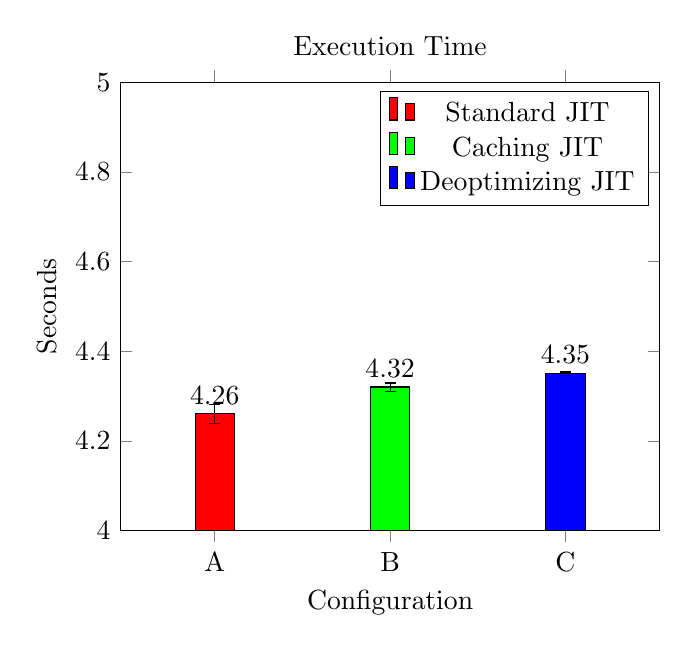
\begin{tikzpicture}
	\begin{axis}[
		ybar,
		title=Execution Time,
		xlabel={Configuration},
		ylabel={Seconds},
		ymin=4,
		ymax=5,
		symbolic x coords={A, B, C},
		xtick={A, B, C},
		bar width=0.5cm,                       %% changed
	   	ybar=-0.5cm,                           %% new
	   	enlarge x limits={abs=1.2cm},
	   	nodes near coords, nodes near coords align={vertical},
	]
\addplot[black, fill=red, error bars/.cd, y dir=both, y explicit] 
	coordinates {
		(A, 4.26) += (0, 0.022) -= (0,0.022)
	}; 
\addplot[black, fill=green, error bars/.cd, y dir=both, y explicit] 
	coordinates {(B,4.32) += (0,0.009) -= (0,0.009)}; 		
\addplot[black, fill=blue, error bars/.cd, y dir=both, y explicit] 
	coordinates {(C,4.35) += (0,0.0035) -= (0,0.0035)}; 
	
\legend{Standard JIT, Caching JIT, Deoptimizing JIT}
\end{axis}
\end{tikzpicture}
\label{fig:5deopts}
\end{figure}	
	
	In this case, the standard language implementation comes out fastest, while the deoptimizing JIT is slowest by a small margin, as expected.
	
	
	\subsection{When To Deoptimize}
	\label{sec:threshold}
	Using the simple replacement strategy described in Section \ref{sec:recompilation} there is one parameter to be tuned: the number of consecutive different types that need to be encountered before the JIT'ed segment is recompiled using new type assumptions.
	
	\begin{figure}[htb]

	\caption{Running time for 200k iterations, 1 class methods with a recompile threshold of 1, 2, 5, 10, and 10000. Plotted on semilog to include the datapoint at 10,000 iterations}
	\begin{tikzpicture}
		\begin{semilogxaxis}[
			title=Execution Time,
			xlabel={Iterations before Recompilation},
			ymin=0.6,
			ymax=0.7,
			ylabel={Seconds},
		   	nodes near coords, nodes near coords align={vertical},
		]
		
	\addplot[color=blue,mark=x] table[x index=0,y index=1, y error=2, col sep=comma] {./data/when_to_deopt.csv};
	
	\end{semilogxaxis}
	\end{tikzpicture}
		\label{fig:deoptimize_threshold}
	\end{figure}	
	

	
	Interestingly, there is very little variation performance as the threshold is varied. The best setting seems to be between 5 and 10, as empirically suggested by Figure \ref{fig:5deopts}. However, unless the threshold is set extremely high there is hardly a any performance difference. At 10,000 side exits the there is a difference of $0.05s$, an approximately $8\%$ performance penalty for spending 10\% of computation traversing the slow path.
	
	This plot reveals that the side exit, interpreter reconstruction, resumption, and return back to the JIT is extremely fast. Given that the fast path of the inline-caching function is extremely short, the big cost to be paid using deoptimization is the time to execute a recompilation via LLVM.


	
\section{Conclusion} 
This report discusses the inclusion of deoptimization into the MysoreScript language. The evaluation focuses on comparing inline caching implementations along with the baseline, non-caching interpreter and JIT.

One strong conclusion is that inline caching is worth it if there are more than a few class methods. However, the hardware is able to execute the $O(n)$ method lookup very efficiently, making the optimizations perform worse with few methods in a class. 

Another is that the time required to recompile a method or closure is relatively high (around 0.15 seconds), meaning it's not worthwhile if frequent recompilations are required. Even just 5 recompilations over a a 4 second runtime place the deoptimizing JIT configuration slower than the alternatives.

The implementation of deoptimization is a little bit incomplete, in that is can be extended to include live variable analysis, reducing the runtime cost of taking the slow path. However, the data also supports that side exit is already very fast -- it is possible another compile time analysis would be detrimental to performance until the cost is amortized over many slow path exits.

\subsection{Future Work}
The most urgent addition to the code base is the ability to have more than one stackmap record per function, which is a rather crippling restriction. Being able to have a fast path with many inline cache hits would make the deoptimizing variant presented much faster in the common case.

A more difficult improvement would be to lift the restriction of only allowing side exits at statement boundaries: this would require a method for returning intermediate results from the compiled execution into non-existent values in the interpreter.






% if have a single appendix:
%\appendix[Proof of the Zonklar Equations]
% or
%\appendix  % for no appendix heading
% do not use \section anymore after \appendix, only \section*
% is possibly needed

% use appendices with more than one appendix
% then use \section to start each appendix
% you must declare a \section before using any
% \subsection or using \label (\appendices by itself
% starts a section numbered zero.)
%


% Can use something like this to put references on a page
% by themselves when using endfloat and the captionsoff option.
\ifCLASSOPTIONcaptionsoff
  \newpage
\fi



% trigger a \newpage just before the given reference
% number - used to balance the columns on the last page
% adjust value as needed - may need to be readjusted if
% the document is modified later
%\IEEEtriggeratref{8}
% The "triggered" command can be changed if desired:
%\IEEEtriggercmd{\enlargethispage{-5in}}

% references section

% can use a bibliography generated by BibTeX as a .bbl file
% BibTeX documentation can be easily obtained at:
% http://mirror.ctan.org/biblio/bibtex/contrib/doc/
% The IEEEtran BibTeX style support page is at:
% http://www.michaelshell.org/tex/ieeetran/bibtex/
%\bibliographystyle{IEEEtran}
% argument is your BibTeX string definitions and bibliography database(s)
%\bibliography{IEEEabrv,../bib/paper}
%
% <OR> manually copy in the resultant .bbl file
% set second argument of \begin to the number of references
% (used to reserve space for the reference number labels box)

\printbibliography

% biography section
% 
\end{document}


